\documentclass[10pt,a4paper]{article}
\usepackage[a4paper]{geometry}

\usepackage[utf8x]{inputenc}
\usepackage{polski}

\usepackage{amsmath}
\usepackage{amssymb}
\usepackage{amsthm}

\usepackage{graphicx}
\usepackage{sidecap}

\usepackage{mathtools}

\theoremstyle{plain}
\newtheorem{theorem}{Twierdzenie}
\newtheorem{lemma}{Lemat}
\theoremstyle{definition}
\newtheorem*{definition}{Definicja}
\newtheorem*{example}{Przykład}

\newcommand{\impl}{\rightarrow}
\newcommand{\N}{\mathbb{N}}

\newcommand{\header}[1]{\noindent\textbf{#1}}

\title{Teoria Programowanie w Logice}
\author{}
\date{Semestr letni 2013}

\begin{document}
\maketitle

\section{Dowody Hilberta}

\header{Język:}

\begin{itemize}
  \item przeliczalnie wiele zmiennych: $\{x_i\}_{i\in\N}$;
  \item funktory: $\impl, \neg$;
  \item zbiór formuł sensownych $S$: najmniejszy zbiór, taki że:
  \begin{enumerate}
    \item $\{x_i\} \subset S$;
    \item jeśli $A, B \in S$, to $A \impl B \in S$ i $\neg A \in S$.
  \end{enumerate}
\end{itemize}

\begin{definition}
$D \subset S$ jest zamknięty na Modus Ponens (MP), gdy
$$\text{jeśli } A \impl B \in D \text{ i } A \in D \text{, to } B \in D.$$
\end{definition}

\begin{lemma}
Jeśli $\alpha$ to pewna rodzina zbiorów zamkniętych na MP,
to $\bigcap\alpha$ jest zamknięty na MP.
\end{lemma}

\begin{lemma}
Jeśli $\alpha$ to pewna rodzina zbiorów zamkniętych na MP, która jest łańcuchem,
to $\bigcup\alpha$ jest zamknięty na MP.
\end{lemma}

\begin{lemma}
Dla każdego $X \subset S$ istnieje najmniejszy zbiór $Y$, taki że
\begin{enumerate}
  \item $X \subset Y$;
  \item $Y$ jest zamknięty na MP.
\end{enumerate}
\end{lemma}

\begin{proof}
$Y = \bigcap \{
  Z \subset S : X \subset Z \text{ i } Z \text { zamknięty na MP}
\}.$
\end{proof}

Taki $Y$ nazywamy \emph{konsekwencją} $X$. ($Cn: 2^S \ni X \mapsto Y \in 2^S$)

\bigskip

\header{Fakty o $Cn$}

\begin{enumerate}
  \item Jeśli $X$ jest zamknięty na MP, to $Cn(X) = X$.
  \item $X \subset Cn(X)$.
  \item Jeśli $X \subset Y$, to $Cn(X) \subset Cn(Y)$.
  \item $Cn(Cn(X)) = Cn(X)$.
  \item $Cn(X) = \bigcup\{
    Cn(Y) : Y \subset X \text{ i } X \text{ jest skończony}
  \}$.
    \begin{proof}
      $\supset$ -- trywialny. $\subset$ -- Wystarczy pokazać, że prawa strona
      jest zamknięta na MP. $A \impl B \in \bigcup \{ \ldots \}$, więc
      $A \impl B \in Cn(Y_1)$, $A \in \bigcup \{ \ldots \}$, więc
      $A \in Cn(Y_2)$, zatem $B \in Cn(Y_1 \cup Y_2)$.
      Na koniec zauważamy, że $Y_1 \cup Y_2$ jest skończonym podzbiorem $X$.
    \end{proof}
  \item $Cn(\emptyset) = \emptyset$.
\end{enumerate}

\bigskip

\header{Alternatywne opisy $Cn$}
\begin{align*}
& H^i: 2^S \to 2^S\\
& H^0(X) = X\\
& H^{n+1}(X) = H^n(X) \cup \{
    B \in S : \exists_{A \in S} (A \impl B \in H^n(X) \text{ i } A \in H^n(X))
  \}\\
& H(X) = \bigcup_{n = 0}^\infty H^n(X)
\end{align*}

\begin{lemma}
$Cn(X) = H(X).$
\end{lemma}

\begin{proof}
$\subset$ -- łatwy, $\supset$ -- przez indukcję ze względu na $n$.
\end{proof}

\begin{definition}[Dowód Hilberta]
$A \in S$ ma dowód Hilberta ze zbioru formuł $X$, gdy istnieje skończony ciąg
formuł $A_0, A_1, \ldots, A_n$, taki że $A_n = A$ i dla każdego $i$:
\begin{itemize}
  \item $A_i \in X$ lub
  \item istnieją $A_j, A_k$, takie że $j, k < i$ i $A_j = A_k \impl A_i$.
\end{itemize}
\end{definition}

%TODO: tu by można jeszcze wspomnieć o drzewowej reprezentacji dowodu.

\begin{definition}[Konsewkencja dowodowa]
$Cn^*(X) := \{ A \in S: A \text{ ma dowód z } X\}$
\end{definition}

\begin{lemma}
$Cn(X) = Cn^*(X)$
\end{lemma}

\begin{proof}
$\supset$ -- przez indukcję ze względu na długość dowodu,
$\subset$ -- przez sklejenie dowodów Hilberta.
%TODO: tę drugą część można by rozpisać dokładniej.
\end{proof}

\bigskip

\begin{definition}[Logika klasyczna]
Niech $L \subset S$ będzie najmniejszym zbiorem zawierającym (dla dowolnych
$A, B, C \in S$)
\begin{itemize}
  \item $K: A \impl (B \impl A)$
  \item $S: (A \impl (B \impl C)) \impl ((A \impl B) \impl (A \impl C))$
  \item $N: (\neg A \impl \neg B) \impl ((\neg A \impl B) \impl A)$
\end{itemize}
oraz zamkniętym na MP.
\end{definition}

\begin{example}
$I: A \impl A \in L$, ponieważ:
\begin{itemize}
  \item $(A \impl (B \impl A)) \impl ((A \impl B) \impl (A \impl A))$
    \quad(aksjomat $S$)
  \item $A \impl (B \impl A)$ \quad(aksjomat $K$)
  \item $(A \impl B) \impl (A \impl A)$ \quad(Modus Ponens)
  \item $(A \impl (C \impl A)) \impl (A \impl A)$ \quad($B := C \impl A$)
  \item $A \impl (C \impl A)$ \quad(aksjomat $K$)
  \item $A \impl A$ \quad(Modus Ponens)
\end{itemize}
\end{example}

\noindent Notacja: $Cn_L(X) := C_n(L \cup X)$.

\begin{theorem}[O dedukcji wprost, TDW]
$b \in Cn_L(X \cup \{a\})$ wtedy i tylko wtedy, gdy $a \impl b \in Cn_L(X)$.
\end{theorem}

\begin{proof}
$\Leftarrow$ -- trywialny. $\Rightarrow$ -- przez indukcję ze względu
na długość dowodu $b$.  %TODO: napisać tę drugą część.
\end{proof}

\begin{theorem}[O dedukcji nie wprost]
Jeśli $z, \neg z \in Cn_L(X \cup \{a, \neg b\})$, to $a \impl b \in Cn_L(X)$.
\end{theorem}

\begin{proof}
\begin{flalign*}
\neg b \impl z &\in Cn_L(X \cup \{a\}) && \text{z TDW}\\
\neg b \impl \neg z &\in Cn_L(X \cup \{a\}) && \text{z TDW}\\
(\neg b \impl \neg z) \impl ((\neg b \impl z) \impl b) 
  &\in L \subset Cn_L(X \cup\{a\}) && \text{aksjomat N}\\
b &\in Cn_L(X \cup \{a\}) && \text{MP} \times 2\\
a \impl b &\in Cn_L(X) && \text{TDW}
\end{flalign*}
\end{proof}

\begin{theorem}
Jeśli $L' \subset S$ jest zbiorem zamkniętym na MP, w którym prawdziwe jest TDW,
to $K, S \in L'$.
\end{theorem}

\begin{proof}
%TODO: napisać dowód.
\end{proof}

\begin{theorem}
Jeśli $L' = Cn(L')$ jest logiką w której zachodzi TDN to $L \subset L'$
\end{theorem}

\begin{proof}
Dla $L'$ jeśli TDN to TDW. \\
($b \rightarrow a \in Cn_{L'}(X) \Rightarrow  a \in Cn_{L'}(X \cup \{b\})$ tryw,
dowodzimy $\Leftarrow$)
\begin{enumerate}
\item $a \in Cn_{L'}(X \cup \{b\}) \subset Cn_{L'} (X \cup \{b, \neg a\})$
\item $\neg a \in Cn_{L'} (X \cup \{b, \neg a\}) $ 
\item $b \rightarrow a \in Cn_{L'}(X)$ (Sprzeczność, TDN)
\end{enumerate}
Zatem TDW, zatem K, S.\\
Udowodnimy teraz że zachodzi również aksjomat S.\\
\begin{enumerate}
\item $b, \neg b \in Cn_{L'}(\{\neg a \rightarrow \neg b, \neg a \rightarrow b, 
\neg a\})$
\item $(\neg a \rightarrow b) \rightarrow a \in Cn_{L'}({\neg a \rightarrow 
\neg b})$ (TDN na dwóch ostatnich formułach)
\item $(\neg a \rightarrow \neg b) \rightarrow 
((\neg a \rightarrow b) \rightarrow a) \in Cn_{L'}(\emptyset) = L'$ (TDW)
\end{enumerate}
\end{proof}

\bigskip

\header{Konstrukcje drzewowe dowodów}
\begin{figure}
\caption{Drzewo MP}
\centering 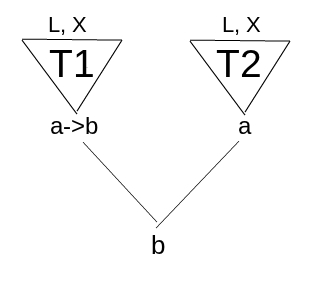
\includegraphics[width=0.3\textwidth]{drzewoMP}
\caption{Drzewo TDW}
\centering 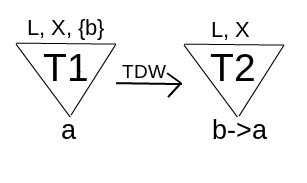
\includegraphics[width=0.4\textwidth]{drzewoTDW}
\caption{Indukcyjna konstrukcja drzewa TDW}
\centering 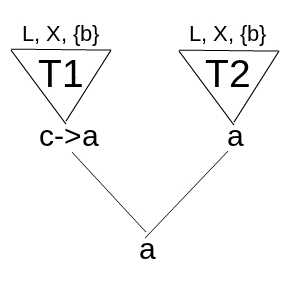
\includegraphics[width=0.25\textwidth]{drzewoMP2}
\centering 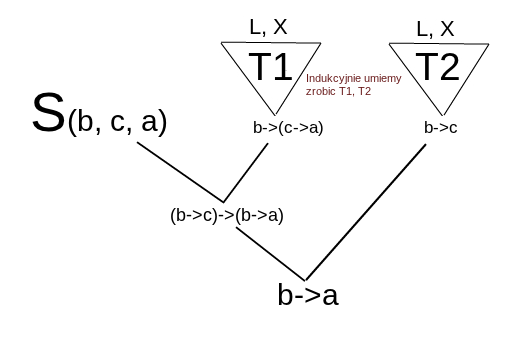
\includegraphics[width=0.5\textwidth]{drzewoTDWindukcyjnie}
\caption{Indukcyjna konstrukcja drzewa TDN}
\centering 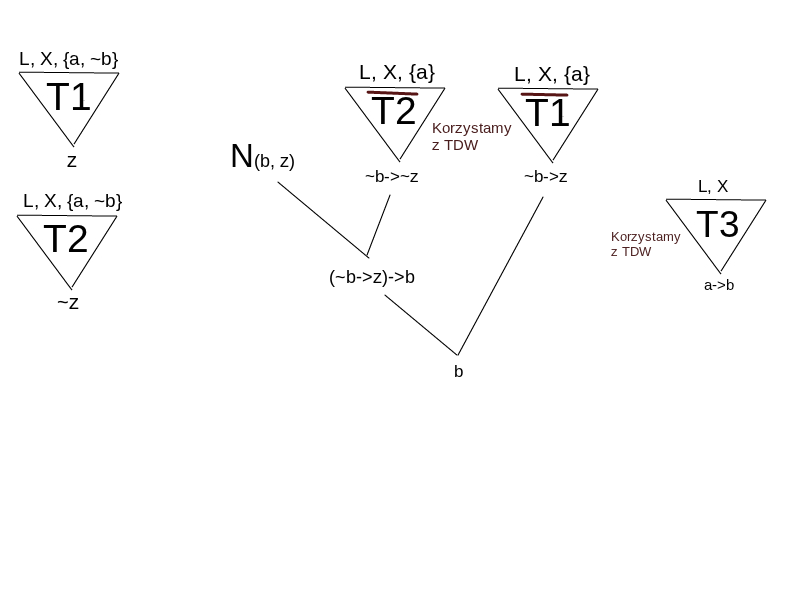
\includegraphics[width=0.7\textwidth]{drzewoTDN}
\end{figure}

Baza indukcji konstrukcji drzewa DTW:
\begin{itemize}
\item T1 jest punktem $a \in L \cup X$, robię $(K_{a, b}$ and $a) 
\Rightarrow b \rightarrow a$
\item T1 jest punktem $b$, robię $((S$ and $K)$ and $K) 
\Rightarrow b \rightarrow b$
\end{itemize}

\newpage

\header{Ćwiczenia}
\begin{enumerate}
\item $\neg \neg p \rightarrow p \in L$?\\
$Cn_{L}(\neg \neg p, \neg p) \xRightarrow{TDN} \neg \neg p \rightarrow p$
\item $p \rightarrow \neg \neg p \in L?$\\
$Cn_{L}(p, \neg \neg \neg p) \Rightarrow Cn_{L}(p, \neg p) \xRightarrow{TDN} 
p \rightarrow \neg \neg p$
\item $(p \rightarrow q) \rightarrow 
((q \rightarrow r) \rightarrow (p \rightarrow r))$?\\
$r \in Cn_{L}({p \rightarrow q, q \rightarrow r, p})$
\item $(p \rightarrow q) \rightarrow (\neg q \rightarrow \neg p)$\\
$Cn_{L}(\{p \rightarrow q, \neg q, \neg \neg p\}) \xRightarrow{TDN} 
(p \rightarrow q) \rightarrow (\neg q \rightarrow \neg p)$
\item $(p \rightarrow q) \rightarrow ((\neg p \rightarrow q) \rightarrow q)$\\
$Cn_{L}(\{p \rightarrow q, \neg p \rightarrow q, \neg q\})$
\begin{itemize}
\item $\neg q$
\item $p \rightarrow q \Rightarrow \neg q \rightarrow \neg p$ (z 4)
\item $\neg p$ (z MP)
\item $\neg p \rightarrow q$
\item $q$ (Sprzeczność)
\end{itemize}
\item Prawo Pierce'a: $((p \rightarrow q) \rightarrow p) \rightarrow p$\\
$Cn_{L}(\{(p \rightarrow q) \rightarrow p, \neg p\})$
\begin{itemize}
\item $\neg p \rightarrow \neg (p \rightarrow q)$ (z kontrapozycji)
\item $\neg p$
\item $\neg (p \rightarrow q)$ (z MP)
\item $\neg (p \rightarrow q) \rightarrow p$
\item $\neg p \rightarrow (p \rightarrow q)$ (z kontrapozycji)
\item $p \rightarrow q$ (z MP, Sprzeczność)
\end{itemize}
\end{enumerate}

\begin{definition}
$X \subset S$ jest \textbf{sprzeczny} gdy $Cn_L(X) = S$.\\
$X \subset S$ jest \textbf{pełny} gdy dla dowolnego $\alpha \in S$ zachodzi 
$\alpha \in Cn_L(X) \vee \neg \alpha \in Cn_L(X)$
\end{definition}

\begin{theorem}[Adolfa Lindenbauma]
Zbiór niesprzeczny da się uzupełnić do niesprzecznego i zupełnego.
\end{theorem}
\begin{proof}
$X$ - niesprzeczny, $S$ - jest przeliczalny, $S = {\alpha_0, \alpha_1, ...}$.\\
Zdefiniujmy ciąg zbiorów:\\
$X_0 = Cn_L(X) \neq S$\\
$X_{i+1} = Cn_L(X_i \cup {\alpha_i}$ gdy $Cn_L(X_i \cup {\alpha_i}) \neq S$\\
$X_{i+1} = X_i$ wpp \\ \\
$X_0 \subset X_1 \subset ...$ \\
$X_i$ - niesprzeczne, zamknięte na MP.\\
$X^{MAX} = \bigcup X_i$, $X^{MAX}$ - niesprzeczne, zamknięte na MP (z lematu 2)
\\ \\
Czy $X^{MAX}$ sprzeczny? Załóżmy że tak, tzn:\\
$\alpha, \neg \alpha \in X^{MAX}$\\
$\alpha \in X_p, \neg \alpha \in X_q$, weźmy $r = max(p, q)$, wówczas:\\
 $\alpha, \neg \alpha \in X_r$, ale $X_r$ miało być niesprzeczne! 
 Zatem $X_{MAX}$ niesprzeczne.\\ \\
Jeśli $X$ sprzeczne to $X$ pełne:\\
$\alpha, \neg \alpha \in Cn_L(X)$ to 
$\alpha \rightarrow (\neg \alpha \rightarrow \beta) \in L$, 
z MP $\beta \in Cn_L(X)$, $\beta$ dowolne. 
\\ \\
Czy $X^{MAX}$ zupełny?\\
Załóżmy że tak nie jest, tzn:\\
$\alpha \not \in X^{MAX}, \neg \alpha \not \in X^{MAX}$\\
Czyli $\forall_p \alpha \not \in X_p \wedge \neg \alpha \not \in X_p$\\
Ale $\alpha \in S$, więc $\alpha = \alpha_p, \neg \alpha = \alpha_q$\\
Bez straty ogólności $p < q$, więc $X_p \subset X_q$

\begin{itemize}
\item $Cn_L(X_q \cup {\alpha}) = S$, $\beta \in Cn_L(X_q \cup {\alpha}) 
\xRightarrow{TDW} (\alpha \rightarrow \beta) \in X_q$
\item $Cn_L(X_q \cup {\neg \alpha}) = S$, 
$\beta \in Cn_L(X_q \cup {\neg \alpha}) \xRightarrow{TDW} 
(\neg \alpha \rightarrow \beta) \in X_q$
\item $(\alpha \rightarrow \beta) \rightarrow (\neg \alpha \rightarrow \beta) 
\rightarrow \beta \in L$
\end{itemize}
z powyższych trzech wynika że $\beta \in X_q$, 
$\beta$ dowolne więc $X_q$ sprzeczne, a miało nie być. 
Zatem sprzeczność i $X^{MAX}$ jest zupełny.

\end{proof}

\end{document}
